% LREC 2026 Example; 
% LREC Is now using templates similar to the ACL ones. 
\documentclass[10pt, a4paper]{article}

\usepackage[review]{lrec2026} % this is the new style
% the 'review' option anonymizes the paper following submission guideline
% the 'final' option produces the camera ready version (non anonymized)
% default version is 'final', so use review option for submission

\title{Title of the LREC 2026 Paper (Title in 14-point Bold, Capitalized in Titlecase)}

\name{Author1, Author2, Author3} 

\address{Affiliation1, Affiliation2, Affiliation3 \\
         Address1, Address2, Address3 \\
         author1@xxx.yy, author2@zzz.edu, author3@hhh.com\\
         \{author1, author5, author9\}@abc.org\\}


\abstract{
Each paper must include an abstract of 150 to 200 words in 9 pt with interlinear spacing of 10 pt. The heading Abstract should be centered, 10 pt bold. This short abstract will also be used for producing the Booklet of Abstracts (PDF) containing the abstracts of all papers presented at the Conference.
 \\ \newline \Keywords{keyword1, keyword2, keyword3} }

\begin{document}

\maketitleabstract

\section{Full Paper Submission}

LREC 2026 has both long and short papers featuring substantial, original, and unpublished research in all aspects of natural language and computation, language resources (LRs) and evaluation, including spoken and sign language and multimodal interaction. Submissions are invited in five broad categories: (i) theories, algorithms, and models, (ii) NLP applications, (iii) language resources, (iv) NLP evaluation and (v) topics of general interest. Submissions that span multiple categories are particularly welcome.   

\paragraph{Submissions may be of three types:}

\begin{itemize}
\item Regular long papers - up to eight (8) pages maximum,* presenting substantial, original, completed, and unpublished work.
\item Short papers - up to four (4) pages,\footnote{Excluding any number of additional pages for references, ethical consideration, conflict-of-interest, as well as data and code availability statements.} describing a small, focused contribution, negative results, system demonstrations, etc.
\item  Position papers - up to eight (8) pages,* discussing key hot topics, challenges and open issues, and cross-fertilization between computational linguistics and other disciplines.
\end{itemize}

Upon acceptance, final versions of long papers will be given one
additional page – up to nine (9) pages of content plus unlimited pages for acknowledgements and references – so that reviewers’ comments can be considered. Final versions of short papers may have up to five (5) pages, plus unlimited pages for acknowledgements and references. All figures and tables that are part of the main text must fit within these page limits for long and short papers.

Papers must be of original, previously-unpublished work. Papers must be \textbf{anonymized to support double-blind reviewing}. Submissions, thus, must not include authors’ names and affiliations. The submissions should also avoid links to non-anonymized repositories: the code should be either submitted as supplementary material in the final version of the paper or as a link to an anonymized repository (e.g., Anonymous GitHub or Anonym Share). Papers that do not conform to these requirements will be rejected without review.

Please use the \texttt{[review]} setting for submissions:

\begin{verbatim}
\usepackage[review]{lrec2026}
\end{verbatim}

This hides the authors and adds page numbers.

\section{How to Produce the \texttt{.pdf}}
\label{sec:append-how-prod}


In order to generate a PDF file out of the LaTeX file herein, when citing language resources, the following steps need to be performed:

\begin{enumerate}
\item \texttt{xelatex your\_paper\_name.tex}
\item \texttt{bibtex your\_paper\_name.aux}
\item \texttt{bibtex languageresource.aux}    *NEW*
\item \texttt{xelatex your\_paper\_name.tex}
\item \texttt{xelatex your\_paper\_name.tex}
\end{enumerate}

From 2026 we are using a sans-serif font TeX Gyre Heros, so you must
install it if you do not have it.  For monospaced font, we use TeX
Gyre Cursor.\footnote{They are available from CTAN in the
  \href{https://ctan.org/pkg/tex-gyre-heros}{tex-gyre-heros} and
  \href{https://ctan.org/pkg/tex-gyre-cursor}{tex-gyre-cursor} packages
    or in TeXLive as \texttt{tex-gyre} and \texttt{tex-cursor}.}  To
  compile, you can use either \textbf{\texttt{pdfLaTeX}},
  \textbf{\texttt{XeLaTeX}} or \textbf{\texttt{LuaLaTeX}}.

\section{Final Paper}

Each final paper should be submitted online. The fully justified text should be formatted according to LREC 2026 style as indicated for the Full Paper submission.

Papers must be up to 5 pages for short papers and 9 pages for long
papers, including figures (plus more pages if needed for references,
ethical consideration, conflict-of-interest, as well as data and code
availability statements).  Length does not depend on the presentation
mode (oral or poster).

\begin{itemize}
\item The paper is in A4-size format, that is 21 x 29.7 cm.
\item The text height is 24.7 cm and the text width 16.0 cm in two
  columns separated by a 0.6 cm space.
\item The font for the entire paper should be Tex Gyre Heros, a
  sans-serif font based Helvetica, with TeX Gyre Cursor for the
  monospaced font.
\item The main text should be 10 pt with an interlinear spacing of 11
  pt.
\item The use of \texttt{lrec2026.sty} will ensure the good formatting.
\end{itemize}



\subsection{General Instructions for the Final Paper}

The unprotected PDF files will appear in the online proceedings directly as received. \textbf{Do not print the page number}.

\section{Page Numbering}

\textbf{Please do not include page numbers in your Paper.} The definitive page numbering of papers published in the proceedings will be decided by the Editorial Committee.

\section{Headings / Level 1 Headings} 

Level 1 Headings should be capitalised in the same way as the main title, and centered within the column. The font used is 12 pt bold. There should also be a space of 12 pt between the title and the preceding section and 3 pt between the title and the following text.

\subsection{Level 2 Headings}

The format of Level 2 Headings is the same as for Level 1 Headings, with the font  11 pt, and the heading is justified to the left of the column. There should also be a space of 6 pt between the title and the preceding section and 3 pt between the title and the following text.

\subsubsection{Level 3 Headings}
\label{level3H}

The format of Level 3 Headings is the same as Level 2, except that the font is  10 pt, and there should be no space left between the heading and the text as in~\ref{level3H}. There should also be a space of 6 pt between the title and the preceding section and 3 pt between the title and the following text.

\section{Citing References in the Text}

\subsection{Bibliographical References}


\begin{table}
\centering
\begin{tabular}{lll}
\hline
\textbf{Output} & \textbf{natbib command} & \textbf{Old command}\\
\hline
\citep{Eco:1990} & \verb|\citep| & \verb|\cite| \\
\citealp{Eco:1990} & \verb|\citealp| & no equivalent \\
\citet{Eco:1990} & \verb|\citet| & \verb|\newcite| \\
\citeyearpar{Eco:1990} & \verb|\citeyearpar| & \verb|\shortcite| \\
\hline
\end{tabular}
\caption{\label{citation-guide} Citation commands supported by the style file. The style is based on the natbib package and supports all natbib citation commands. It also supports commands defined in previous style files for compatibility.}
\end{table}

Table~\ref{citation-guide} shows the syntax supported by the style files. We encourage you to use the natbib styles.
You can use the command \verb|\citet| (cite in text) to get ``author (year)'' citations, like this citation to a paper by \citet{CastorPollux-92}. You can use the command \verb|\citep| (cite in parentheses) to get ``(author, year)'' citations \citep{CastorPollux-92}. You can use the command \verb|\citealp| (alternative cite without parentheses) to get ``author, year'' citations, which is useful for using citations within parentheses (e.g. \citealp{CastorPollux-92}).

When several authors are cited, those references should be separated with a semicolon: \cite{Martin-90,CastorPollux-92}. When the reference has more than three authors, only cite the name of the first author followed by ``et.\ al.'', e.g. \citet{Superman-Batman-Catwoman-Spiderman-00}.

\subsection{Language Resource References}

\subsubsection{When Citing Language Resources}

As you may know, LREC introduced a separate section on Language
Resources citation to enhance the value of such assets. When citing
language resources, we recommend to proceed in the same way as for
bibliographical references. Please make sure to compile your Language
Resources stored as a \texttt{.bib} file \textbf{separately}. This
produces the required \texttt{.aux} and \texttt{.bbl} files.  See
Section~\ref{sec:append-how-prod} for details on how to produce this
with bibtex.

A language resource should be cited inline as, for example,
\citetlanguageresource{Speecon}, or \citetlanguageresource{EMILLE} or
parenthetically \citeplanguageresource{ItalWordNet}.  All online
language resources should have a persistent identifier (pid), following the \href{https://doi.org/10.15497/RDA00040}{Tromsø recommendations for citation of research data in linguistics}.

Please add either an ISLRN (International Standard Language Resource
Number) in the \texttt{islrn} field or some other url in the
\texttt{pid} field.  This will be hyperlinked and shown in the
bibliography.  We give an example in the entry for \texttt{ItalWordNet} which you can see in \path{languageresource.bib}.
  



  
\section{Figures \& Tables}

\subsection{Figures}

All figures should be centred and clearly distinguishable. They should never be drawn by hand, and the lines must be very dark in order to ensure a high-quality printed version. Figures should be numbered in the text, and have a caption in  10 pt underneath. A space must be left between each figure and its respective caption. 

Example of a figure:

\begin{figure}[!ht]
\begin{center}
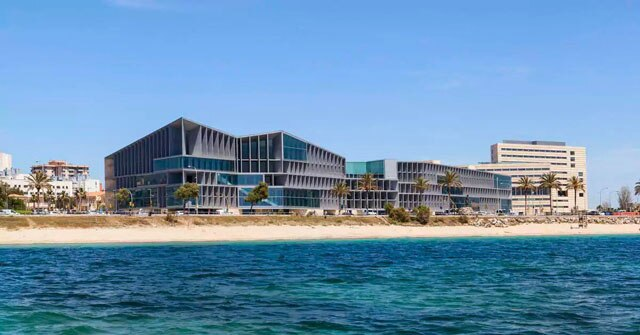
\includegraphics[width=\columnwidth]{home-palacio.jpg}
\caption{The caption of the figure.}
\label{fig.1}
\end{center}
\end{figure}

Figure and caption should always appear together on the same page. Large figures can be centered, using a full page.

\subsection{Tables}

The instructions for tables are the same as for figures.

\begin{table}[!ht]
\begin{center}
\begin{tabularx}{\columnwidth}{|l|X|}

      \hline
      Level&Tools\\
      \hline
      Morphology & Pitrat Analyser\\
      \hline
      Syntax & LFG Analyser (C-Structure)\\
      \hline
     Semantics & LFG F-Structures + Sowa's\\
     & Conceptual Graphs\\
      \hline

\end{tabularx}
\caption{The caption of the table}
 \end{center}
\end{table}

\section{Footnotes}

Footnotes are indicated within the text by a number in superscript\footnote{Footnotes should be in  9 pt, and appear at the bottom of the same page as their corresponding number. Footnotes should also be separated from the rest of the text by a 5 cm long horizontal line.}.

\section{Copyrights}

The Language Resources and Evaluation Conference (LREC) Proceedings are published by the European Language Resources Association (ELRA). They are available online from the conference website.

ELRA's policy is to acquire copyright for all LREC contributions. In assigning your copyright, you are not forfeiting your right to use your contribution elsewhere. This you may do without seeking permission and is subject only to normal acknowledgment to the LREC proceedings. The LREC Proceedings are licensed under CC-BY-NC, the Creative Commons Attribution-Non-Commercial 4.0 International License.


\section{Conclusion}

Your submission of a finalized contribution for inclusion in the LREC Proceedings automatically assigns the above copyright to ELRA.

\section{Acknowledgements}

Place all acknowledgments (including those concerning research grants and funding) in a separate section at the end of the paper.

\section{Optional Supplementary Materials}

Appendices or supplementary material (software and data) will be allowed ONLY in the final, camera-ready version, but not during submission, as papers should be reviewed without the need to refer to any supplementary
materials.

Each \textbf{camera ready} submission can be accompanied by an appendix usually being included in a main PDF paper file, one \texttt{.tgz} or \texttt{.zip} archive containing software, and one \texttt{.tgz} or \texttt{.zip} archive containing data.

We encourage the submission of these supplementary materials to improve the reproducibility of results and to enable authors to provide additional information that does not fit in the paper. For example, preprocessing decisions, model parameters, feature templates, lengthy proofs or derivations, pseudocode, sample system inputs/outputs, and other details necessary for the exact replication of the work described in the paper can be put into the appendix. However, the paper submissions must remain fully self-contained, as these supplementary materials are optional, and reviewers are not even asked to review or download them. If the pseudo-code or derivations, or model specifications are an essential part of the contribution, or if they are important for the reviewers to assess the technical correctness of the work, they should be a part of the main paper and not appear in the appendix.

\subsection{Appendices}

Appendices are material that can be read and include lemmas, formulas, proofs, and tables that are not critical to the reading and understanding of the paper, as in \href{https://acl-org.github.io/ACLPUB/formatting.html#appendices}{*ACLPUB}. It is  highly recommended that the appendices should come after the references; the main text and appendices should be contained in a `single' manuscript file, without being separately maintained. Letter them in sequence and provide an informative title: \textit{Appendix A. Title of Appendix}


\subsection{Extra space for ethical considerations and limitations}

Please note that extra space is allowed after the 8th page (4th page for short papers) for an ethics/broader impact statement and a discussion of limitations. At submission time, if you need extra space for these sections, it should be placed after the conclusion so that it is possible to rapidly check that the rest of the paper still fits in 8 pages (4 pages for short papers). Ethical considerations sections, limitations, acknowledgments, and references do not count against these limits. For camera-ready versions, nine pages of content will be allowed for long (5 for short)
papers.

\section{Providing References}

\subsection{Bibliographical References} 

Bibliographical references should be listed in alphabetical order at the end of the paper. The title of the section, ``Bibliographical References'', should be a Level 1 Heading. The first line of each bibliographical reference should be justified to the left of the column, and the rest of the entry should be indented by 0.35 cm.

The examples provided in Section~\ref{sec:reference} (some of which are fictitious references) illustrate the basic format required for papers in conference proceedings, books, journal articles, PhD theses, and books chapters.

\subsection{Language Resource References}

Language resource references should be listed in alphabetical order at the end of the paper.

\nocite{*}
\section{Bibliographical References}\label{sec:reference}

\bibliographystyle{lrec2026-natbib}
\bibliography{lrec2026-example}

\section{Language Resource References}
\label{lr:ref}
\bibliographystylelanguageresource{lrec2026-natbib}
\bibliographylanguageresource{languageresource}


\end{document}

%%% Local Variables:
%%% mode: latex
%%% TeX-master: t
%%% End:
